%
%  template.tex
%
%  Created by Drew Conway on 2011-01-06
% 
%
\documentclass[xcolor=dvipsnames, 9pt]{beamer}

\usepackage{amssymb}
\usepackage{amsfonts}
\usepackage{amsmath}
\usepackage{hyperref}
\usepackage{natbib}
\usepackage{color}
\usepackage{pdfsync}
\usepackage{chancery}
\usepackage{movie15}
\usepackage{pgfpages}
\usepackage{fancyvrb}
\usepackage{colortbl}
\usepackage{multirow}

\usepackage{graphicx}
\graphicspath{{../../images/figures/}{../../images/logos/}{../../images/graphs/}/}

\usepackage{beamerthemesplit}
\usetheme{Copenhagen}
\definecolor{title}{RGB}{128,148,182}
\usecolortheme[named=title]{structure} 
\setbeamertemplate{headline}{}
\setbeamertemplate{navigation symbols}{}
\setbeamertemplate{itemize items}[triangle]
\setbeamertemplate{enumerate items}[default]
\setbeamertemplate{footline}[page number]{}
%\setbeameroption{show notes on second screen}


\usepackage{listings}
%\usepackage{listings,arev}
\definecolor{keywords}{RGB}{128,148,182}
\definecolor{comments}{RGB}{60,179,113}
\lstset{numbers=left,
        showstringspaces=false,
        numberstyle=\tiny,
        %frame=leftline,
        numbersep=4.5pt,
  keywordstyle=\color{keywords}\bfseries,
  commentstyle=\color{YellowOrange}\emph
}

\newenvironment{code}{\begin{semiverbatim} \begin{footnotesize}}
{\end{footnotesize}\end{semiverbatim}}


\newcommand{\R}{\mathbb{R}}
\renewcommand{\d}{\mathsf{d}}
\newcommand{\dd}{\partial}
\newcommand{\E}{\mathsf{E}}
\newcommand{\bb}{\mathbf}

\title{Strata Data Bootcamp: Slide Template}
\author{Joseph Adler, Drew Conway, Jake Hofman, Hilary Mason}
\date{February 1, 2011}

\begin{document} 

\begin{frame}[plain]
  \titlepage 
  
  \tiny
  \href{http://creativecommons.org/licenses/by-sa/3.0/us/}{
\includegraphics[width=1cm]{ccbysa}}

  Creative Commons Attribution-Share Alike 3.0
\end{frame}

\begin{frame}
	\frametitle{Review of schedule}
	\begin{enumerate}
	   \item Introductions and admin (30 minutes)
	   \item Working with image data (09:30 - 90 minutes)
	   \item Working with text data (11:00 - 90 minutes)
	   \item LUNCH (12:30-13:30)
	   \item Big Data (90 minutes)
	   \item Data mashups (15:00 - 60 mins)
	   \item Concluding panel discussion (16:00 - 60 mins)
	\end{enumerate}
\end{frame}

\begin{frame}[fragile]
    \frametitle{Code Examples}
    This is how I write a \texttt{Python} example...
    \begin{lstlisting}[language=Python]
>>> import networkx as nx
>>> G=nx.Graph()
>>> G.add_edges_from([(1,2),(1,3)])
>>> G.add_node("spam")
    \end{lstlisting}
\vspace{2mm}
    This is how I write an \texttt{R} example...}
    \begin{lstlisting}[language=R]
> library(igraph)
> g <- graph( c(0,1, 1,2, 3,4, 5,6) )
> g
Vertices: 7 
Edges: 4 
Directed: TRUE 

Edges:
[0] 0 -> 1
[1] 1 -> 2
[2] 3 -> 4
[3] 5 -> 6
    \end{lstlisting}
\end{frame}

\begin{frame}[fragile]
    \frametitle{Tables and graphs}
    \begin{columns}
        \column{.5\textwidth}
        This is how I make tables...\vspace{2mm}
        \begin{tabular}{l|ll}
            Fruit & Color & Delicious \\ \hline\hline
            Banana & Yellow  & Yes \\
            Apple & Multi & Yes \\
            Orange & Orange & Yes
        \end{tabular}
        \column{.5\textwidth}
        This is how I draw figures...
        \begin{figure}
            \centering
            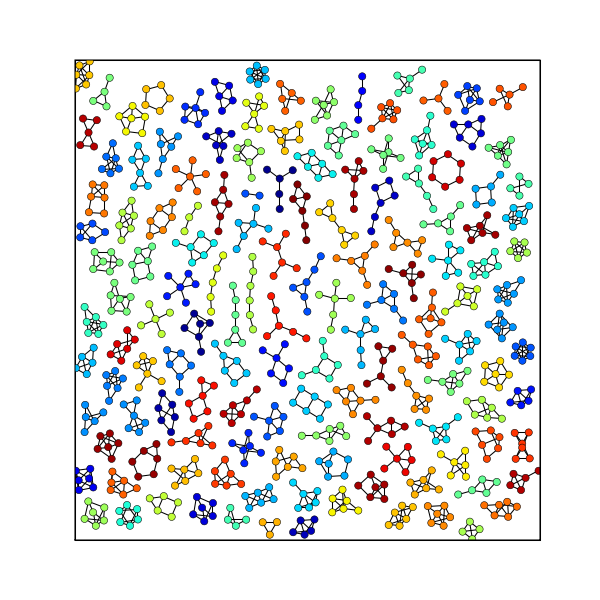
\includegraphics[width=5cm]{atlas.png}
            \caption{The small graph atlas}
        \end{figure}
    \end{columns}
\end{frame}


\end{document}
